\documentclass[14 pt]{extarticle}

	\usepackage[frenchb]{babel}
	\usepackage[utf8]{inputenc}  
	\usepackage[T1]{fontenc}
	\usepackage{amssymb}
	\usepackage[mathscr]{euscript}
	\usepackage{stmaryrd}
	\usepackage{amsmath}
	\usepackage{tikz}
	\usepackage[all,cmtip]{xy}
	\usepackage{amsthm}
	\usepackage{varioref}
	\usepackage{geometry}
	\geometry{a4paper}
	\usepackage{lmodern}
	\usepackage{hyperref}
	\usepackage{array}
	 \usepackage{fancyhdr}
	 \usepackage{float}
\renewcommand{\theenumi}{\alph{enumi})}
	\pagestyle{fancy}
	\theoremstyle{plain}
	\fancyfoot[C]{} 
	\fancyhead[L]{Contrôle}
	\fancyhead[R]{6 novembre 2024}\geometry{
 a4paper,
 total={190mm,257mm},
 left=10mm,
 top=20mm,
 }
	
	
	\title{Contrôle Chapitre 2}
	\date{}
	\begin{document}

 Nom : \\
 Prénom : 
 \subsection*{Exercice 1 (3 points)}
 Calculez, \emph{en détaillant les étapes} : 
 \begin{enumerate}
 \item $7  + 8 \times 4$
 \item $(14 -1 + 3) \div 2 +2 $
 \item $ (10 + 6)\div 2 \times2$
 \end{enumerate}
 
 \subsection*{Exercice 2 (9 points)}
 
 Tracez les symétriques des figures suivantes par rapport au point $D$ et par rapport au point $E$. (Laissez vos traits de construction en pointillés).
 
 \begin{figure}[H]
 \center
 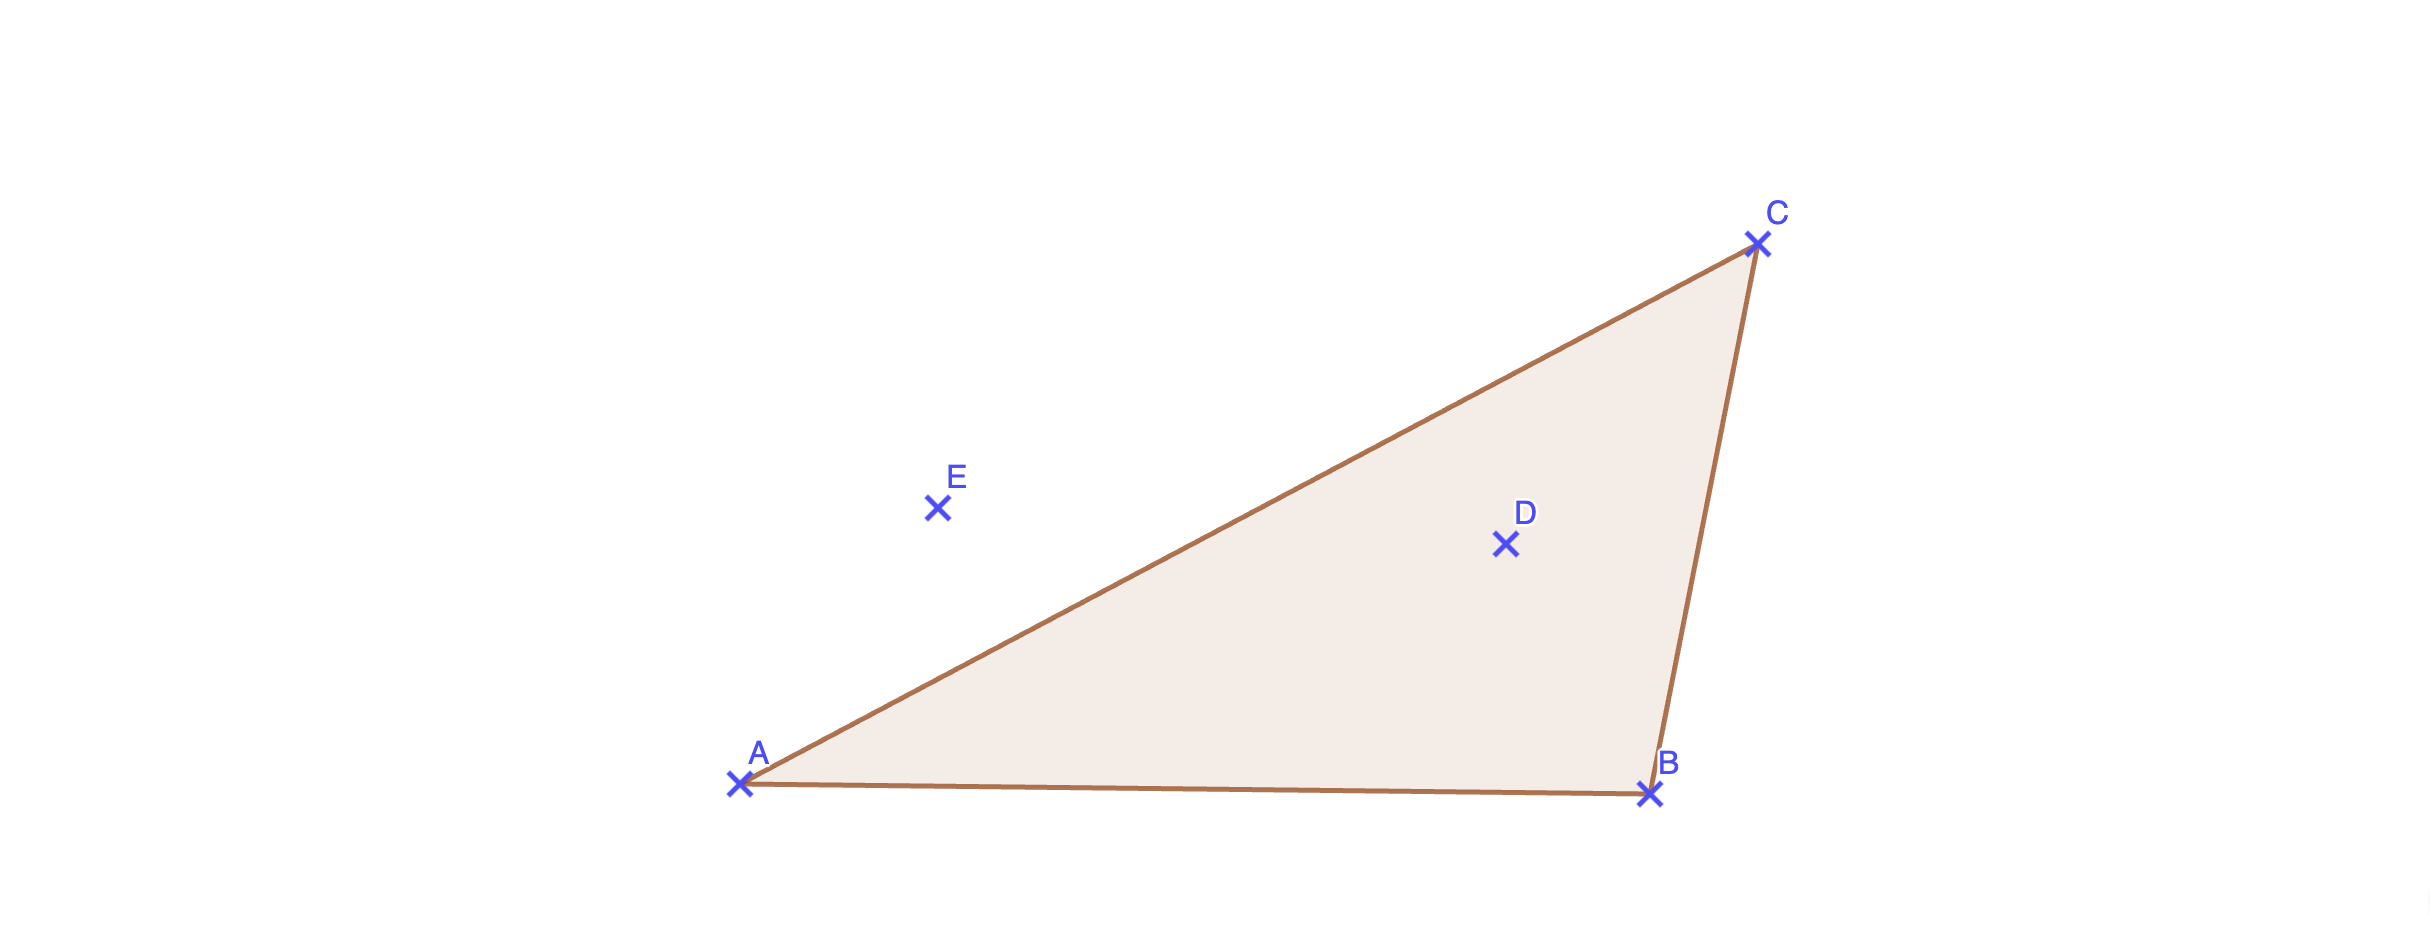
\includegraphics[width = 19 cm]{Exo2}
 \end{figure}
 
 \subsection*{Exercice 3 (3 points)}
 Dans les figures suivantes, citez les axes et centres de symétrie s'il y en a. 
 
 
\includegraphics[width = 5 cm]{ecosse.png}\ \ \ \ 
 
\includegraphics[width = 5 cm]{Micronesie.png}\ \ \ \ 
 
\includegraphics[width = 5 cm]{UnionJack.png}
 \newpage
 \subsection*{Exercice 4 (5 points)}

On considère un quadrilatère ABCD dont les diagonales se croisent en $O$. On suppose que $O$ est le milieu des deux diagonales.
\begin{enumerate}
\item Faire une figure à main levée. 
\item Montrer que les points A et C sont symétriques par rapport à O. 
\item Montrer que les points B et D sont symétriques par rapport à O. 
\item En déduire que $(AB)//(CD)$ et que $(BC)//(AD)$.
\end{enumerate}



 	\end{document}
